\chapter{Benchmarks}\label{chap:benchmarks}

Soup includes a series of benchmarks designed to reproduce different real world
scenarios where usage of Soup might be appropriate. The Lobsters and Vote
benchmarks existed prior to this thesis, while the Recovery and Replay
benchmarks were explicitly built to highlight the positive and negative impact
the features developed in this thesis have on Soup.

\newpage

\section{Hardware}

% TODO: write something here

\subsection{Server setup 1: SSD}\label{sec:server-1}

Unless otherwise specified, benchmarks are run on Dell PowerEdge R430 server
with two Intel Xeon E5-2660 v3 CPUs and a total of 20 physical and 40 logical
cores. The server has 64GB of DDR4 RAM running at a speed of 2200MHz, with two
solid-state drives: a Samsung SSD 850 PRO and an Intel SSD S3710.

\subsection{Server setup 2: EC2 NVMe SSD}\label{sec:server-2}

Some of the benchmarks require the workload generator and clients to be
separated on a different machine than Soup itself. For these cases, the
benchmarks are run on Amazon's Elastic Compute Cloud (EC2)
instances\furl{https://aws.amazon.com/ec2/instance-types/}, typically with the
workload generator running on a machine with a large number of cores and the
Soup server itself running on a server with fewer and faster cores.

When Soup needs access to fast durable storage, an \code{m4.10xlarge} instance
is used for the clients and an \code{i3.4xlarge} instance is used for the Soup
workers. The \code{m4.10xlarge} server uses an Intel Xeon E5-2686 CPU with 40
logical cores and 160 GB of RAM.\@ The \code{i3.4xlarge} uses the same CPU as
the \code{m4}, but is backed by NVMe SSDs capable of extremely high throughput
I/O.

\subsection{Server setup 3: EC2 RAM Disk}\label{sec:server-3}

Similar to the setup in the previous section, the third setup makes use of two
servers hosted on Amazon EC2---this time without fast durable storage. Instead,
an \code{m5.12xlarge} and a \code{c5.4xlarge} is used. Both make use of newer
Intel Xeon Platinum processors, with 48 cores and 192GB RAM on the \code{m5} and
16 cores and 32GB RAM on the \code{c5}.

\section{Lobsters}\label{sec:lobsters}

Lobsters\furl{http://lobste.rs/} is a news aggregation website where users post,
vote, and comment on links and discussions. Soup uses Lobsters to showcase the
performance advantages of Soup in a real-world application. While Lobsters is
built with Ruby on Rails, the Soup benchmark runs MySQL queries normally issued
by Lobsters directly against Soup, using the MySQL protocol shim described in
section~\ref{sec:mysql-shim}. This avoids the overhead of Ruby and Ruby on
Rails, which quickly become bottlenecks when the Lobsters traffic is scaled
beyond its regular workload.

Whereas the other benchmarks focus on individual writes and reads, the Lobsters
benchmark is measured in page views, where different pages execute a series of
write and read queries. The distribution of page views is modeled after real
Lobsters production traffic, to ensure the queries executed best resemble a real
Lobsters setup.

\begin{figure}[H]
  \centering
  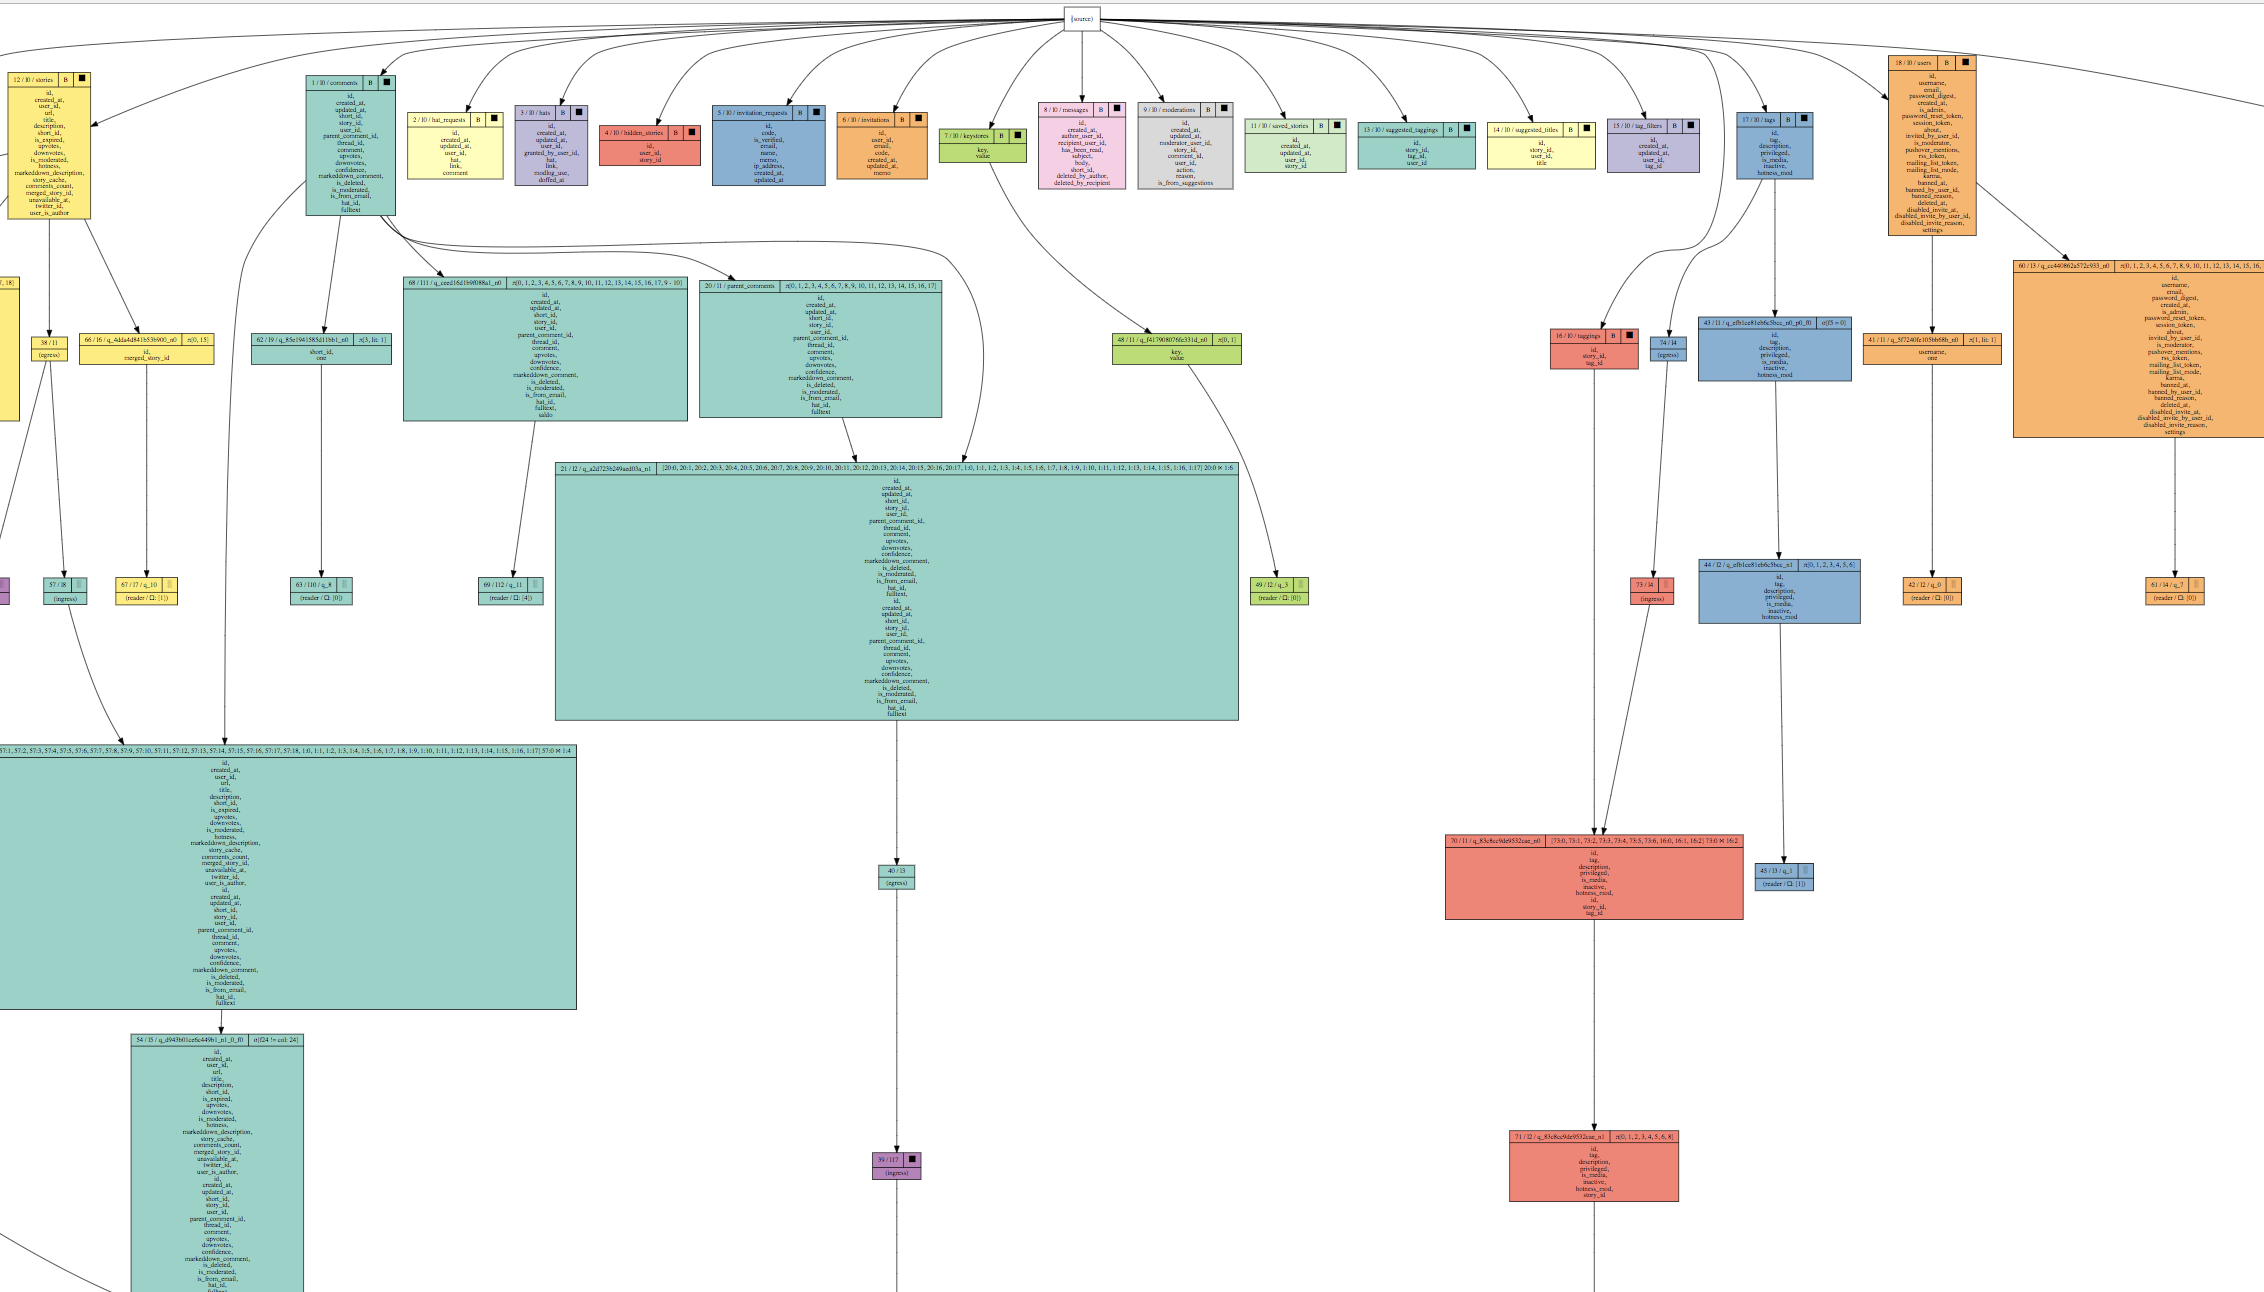
\includegraphics[width=\textwidth]{lobsters}
  \caption{\
    A subset of the Soup data-flow graph used to run the Lobsters benchmark.
  }\label{fig:lobsters-graph}
\end{figure}

The regular Lobsters queries rely on manual materializations and other
optimizations to reach decent performance using MySQL.\@ Part of Soup's goal is
to let developers write ``natural'' queries, without caching or other
denormalizing optimizations, and some of the Lobsters queries have been
rewritten to better highlight this.

\section{Vote}\label{sec:vote}

The Lobsters benchmark includes a wide variety of different queries, making it
difficult to narrow down bottlenecks in Soup's query processing performance. The
vote benchmark solves this by focusing on the most frequently run query in
Lobsters, reading stories and their corresponding vote counts.

\begin{listing}[H]
  \begin{minted}[frame=lines]{sql}
CREATE TABLE Article (id int, title varchar(255), PRIMARY KEY(id));
CREATE TABLE Vote (article_id int, user int);

QUERY ArticleWithVoteCount:
  SELECT Article.id, title, VoteCount.votes AS votes
  FROM Article
  LEFT JOIN (
    SELECT Vote.article_id, COUNT(user) AS votes
    FROM Vote
    GROUP BY Vote.article_id
  ) AS VoteCount
  ON (Article.id = VoteCount.article_id) WHERE Article.id = ?;
  \end{minted}

  \caption{The schema used by the vote benchmark.}\label{lst:vote}
\end{listing}

The database is prepopulated with a series of articles, letting the write
portion of the benchmark focus on writing votes, where each vote is assigned to
an article following a uniform distribution. The vote benchmark runs either
locally against a single Soup instance, or against a cluster of Soup workers.

% TODO: why this thesis only runs benchmarks on a single souplet

\subsection{Open-loop}\label{sec:vote-open-loop}

In a closed-loop benchmark, a new request is issued when the previous completes.
With open-loop, requests are instead issued independently, resulting in a model
more closely resembling a real-world scenario~\cite{open-loop}. Soup's vote
benchmark relies on a \textit{partially} open-loop setup, where load is
generated by clients based on a specified distribution, while maintaining a
capped queue of outstanding requests. This prevents reductions in measurements
during slower processing periods, where a closed-loop benchmark would issue far
fewer requests than an open-loop one.

Two latency measures are recorded during the vote benchmark: the time it takes
for a single batch to be processed (\textit{sojourn} time), and the time it
takes from the request is generated to it completes (\textit{batch processing}
time). The former is usually higher than the latter, as it includes the delay
from the request is queued until it is processed by the system.

\section{Replay}\label{sec:bench-replay}

Part of the promise of Soup is to avoid expensive computations for reads, by
moving most of the workload to the write portion of the system. Read queries
trigger replays for keys initially, while later requests are served directly by
partially materialized state further down the graph. This makes it difficult to
reason about the read performance of Soup's base nodes, as only a small portion
of reads are bound to be served by the base nodes at all.

This is where the replay benchmark comes in. Instead of possibly reading the
same keys multiple times, the replay benchmark ensures that each key is only
ever read \textit{once}, triggering a replay from the base nodes. Additionally,
the schema is far simpler than in the vote benchmark, with a single base node
and different variants of the same query. This avoids excessive computation in
partial nodes in the lower portions of the graph, and focuses the main portion
of the benchmark on state processing at the base node level.

\begin{listing}[H]
  \begin{minted}[frame=lines]{sql}
CREATE TABLE TableRow (
  id int, c1 int, c2 int, c3 int, c4 int,
  c5 int, c6 int, c7 int, c8 int, c9 int,
  PRIMARY KEY(id)
);

/* Primary key reads: */
QUERY ReadRow: SELECT * FROM TableRow WHERE id = ?;

/* Secondary key reads */
QUERY query_c1: SELECT * FROM TableRow WHERE c1 = ?;
/* .. */
QUERY query_c9: SELECT * FROM TableRow WHERE c9 = ?;
  \end{minted}

  \caption{The schema used by the replay benchmark.}\label{lst:replay}
\end{listing}

While trifling for the regular Soup base node implementation, the difference
between reading from a primary and secondary index might be consequential with
persistent base nodes (see chapter~\ref{chap:persistent-bases}). To correctly
assess this difference, the replay benchmark includes the possibility of reading
either from a primary or a secondary index. The row size is also slightly larger
than in the other benchmarks, ensuring that the base nodes actually have to read
a fair share of data from state.

Prior to reading, Soup is populated with a given number of rows, which it then
reads a uniform, and smaller, sample of. With persistent base nodes, the
benchmark terminates after prepopulation, followed by a recovery step, to ensure
that data is served directly from durable storage. The file system cache is also
cleared after recovery and between subsequent benchmark runs.

\section{Recovery}\label{sec:bench-recovery}

The final benchmark measures the recovery time of our voting application, using
the schema described in listing~\ref{lst:vote}. The database is first populated
with a series of articles and votes, before being shut down and recovered from.

The benchmark produces two measures: initial and total recovery time. The former
records how long it takes for the first read to return correct data, while the
latter only finishes when up-to-date data is returned from \textit{all} keys.
